% *********************************************************************
% © 2016–2025 Jeremy Sylvestre
%
% Permission is granted to copy, distribute and/or modify this document
% under the terms of the GNU Free Documentation License, Version 1.3 or
% any later version published by the Free Software Foundation; with no
% Invariant Sections, no Front-Cover Texts, and no Back-Cover Texts. A
% copy of the license is included in the appendix entitled “GNU Free
% Documentation License” that appears in the output document of this
% PreTeXt source code. All trademarks™ are the registered® marks of
% their respective owners.
%
% *********************************************************************
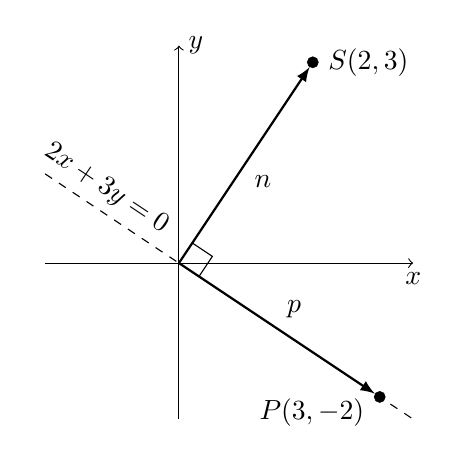
\begin{tikzpicture}[
	point/.style={circle,draw,very thin,fill,inner sep=0pt,minimum size=4pt},
	vector/.style={-latex},
	scale=0.85
]


	\draw[->] (-2,0) to (3.5,0) node[below] {$x$};
	\draw[->] (0,-2.333) to (0,3.25) node[right] {$y$};

	\draw[dashed] (-2,1.333) to node[above,very near start,sloped,xshift=0.05cm] {$2x+3y=0$} (3.5,-2.333);
	\node[point] at (3,-2) (p) [label={[yshift=-0.2cm]left:{$P(3,-2)$}}] {};
	\draw[vector,thick] (0,0) to node[above right] {$\uvec{p}$} (p);
	\node[point] at (2,3) (s) [label=right:{$S(2,3)$}] {};
	\draw[vector,thick] (0,0) to node[below right] {$\uvec{n}$} (s);
	\draw (0.2,0.3) to (0.5,0.1) to (0.3,-0.2);

\end{tikzpicture}
